% Technical report (English). Build: bash docs/report/build.sh
\documentclass[10pt,a4paper,twocolumn]{article}
\usepackage[margin=17mm,columnsep=6mm]{geometry}
\usepackage{amsmath,amssymb}
\usepackage{booktabs}
\usepackage{graphicx}
\usepackage{xcolor}
\usepackage{tikz}
\usetikzlibrary{positioning,arrows.meta,fit,calc}
\usepackage[font=small,labelfont=bf]{caption}
\usepackage{enumitem}
\setlist{nosep,leftmargin=*}
\usepackage{xeCJK}
\setCJKmainfont[Path=fonts/,BoldFont=NotoSerifJP-Bold.otf]{NotoSerifJP-Regular.otf}
\usepackage[colorlinks=true,linkcolor=blue!50!black,citecolor=blue!50!black,urlcolor=blue!50!black]{hyperref}
\newcommand{\pt}{\,pt}
\setlength{\emergencystretch}{1.5em}

\title{\bfseries Teaching a Flow-Matching TTS to Read Kanji:\\
Text-Only Self-Distillation of the Text Encoder of Irodori-TTS}
\author{Claude (Anthropic)\thanks{Claude (Opus 5.5), working in Claude Code, planned and implemented
the experiments, ran them, analyzed the results and wrote this report. Takuma Mori proposed the idea of
fine-tuning only the text encoder with text-only data, set the goals (fewer on/kun swaps, no benchmark
data in the production model), steered the data choices, did the listening tests and decided the
releases.}\qquad Takuma Mori}
\date{{\small Technical report, October 2026}\\
{\small\url{https://github.com/takuma104/Irodori-TTS-Experiments}}}

\begin{document}
\maketitle

\begin{abstract}
Japanese text-to-speech (TTS) has to choose among several readings of most kanji, such as
on'yomi and kun'yomi, from context. We study Irodori-TTS-v4.1-Small, a rectified-flow
diffusion transformer (DiT) that reads raw Japanese text through a pretrained ModernBERT
encoder. On the JKYB-Parakeet benchmark, most of its reading errors are systematic. Writing
the target word in katakana fixes 85\% of them, so the frozen acoustic model can already
pronounce the right reading; the text path chooses the wrong one. We turn this into
supervision. The frozen model, given the katakana sentence, is the teacher. A trainable copy
of the text path (the top 4 BERT layers and the projector), given the kanji sentence, is the
student. The student is trained so that the frozen DiT's velocity and duration predictions
match the teacher's. No speech recordings are needed: target words come from dictionaries,
and their sentences from an LLM, Wikipedia and the ruby (reading annotations) of Aozora Bunko.
Together with preservation losses, target-window loss weighting, more sentences per word and
checkpoint averaging, the released model raises target reading accuracy on held-out Aozora
Bunko ruby from 62.5\% to 67.5\% and on JKYB-Parakeet from 94.0\% to 95.7\%. General sentences
show no measurable regression. We also report where the method stops helping (untrained
words, memorization of sentences) and discuss its use for other languages, such as Mandarin
polyphonic characters.
\end{abstract}

\section{Introduction}
Most kanji have several readings, and the reading depends on the word and the context:
生 is \emph{sei} in 生活, \emph{nama} in 生ビール, \emph{i} in 生きる. Classic
Japanese TTS front-ends resolve readings with a morphological analyzer and a pronunciation
dictionary~\cite{mecab,unidic,sudachi}. Recent end-to-end models instead read raw text, so the
reading is decided implicitly inside the network and only for words that the paired speech
data covered.

Irodori-TTS-v4.1-Small~\cite{irodori} is such a model. On JKYB-Parakeet~\cite{jkyb,jkybp}, a
benchmark of 13,536 sentences each with a tagged target word, it reads 93.9\% of the targets
correctly. When we listened to its errors, swaps between on'yomi and kun'yomi (音訓の取り違え)
were the most noticeable. This report describes how we reduced such errors
\emph{without new speech data and without touching the acoustic model}:
\begin{itemize}
\item a diagnosis showing that the errors come from the text path (\S\ref{sec:diag});
\item kana-substitution self-distillation, which fine-tunes only the text encoder (\S\ref{sec:method});
\item a data pipeline built from dictionaries, an LLM, Wikipedia and Aozora Bunko ruby, which
  does not use the benchmark (\S\ref{sec:data});
\item findings on loss dilution, memorization versus sentence variety, drift on untrained words
  and checkpoint averaging (\S\ref{sec:exp}).
\end{itemize}
The checkpoint is released on Hugging Face\footnote{\url{https://huggingface.co/takuma104/Irodori-TTS-v4.1-Small-Yomi}}
and works with the original inference code.

\section{Irodori-TTS and Echo-TTS}\label{sec:arch}
\textbf{Echo-TTS}~\cite{echo} is a multi-speaker TTS model. A diffusion transformer generates
the continuous latents of an audio autoencoder with rectified flow~\cite{rf,fm}, an approach
also known as flow matching. Text, as UTF-8 bytes, goes through a bidirectional transformer
encoder. A separate encoder reads patched latents of up to two minutes of reference speech. In
each decoder block, the keys and values of the text and speaker encoders are concatenated with
those of the denoiser, so that one attention covers self-attention and conditioning. Timesteps
condition the blocks through a low-rank adaptive layer norm (AdaLN). Text and speaker
conditions are dropped independently during training, which enables classifier-free
guidance (CFG)~\cite{cfg} with separate text and speaker scales.

\textbf{Irodori-TTS}~\cite{irodori} follows this design closely. Table~\ref{tab:arch} lists the
components of v4.1-Small:
\begin{itemize}
\item \textbf{Target:} 32-dimensional latents of a DACVAE codec~\cite{dacvae,dac} at 25\,Hz,
  decoded to 48\,kHz audio.
\item \textbf{DiT:} the RF-DiT (12 blocks, width 1280) uses joint attention, low-rank AdaLN,
  half-RoPE and SwiGLU.
\item \textbf{Text:} instead of a byte encoder, v4 uses a pretrained Japanese
  ModernBERT~\cite{modernbert,modernbertja}, fine-tuned with the model. Its
  states go through a residual-MLP projector and an RMSNorm (\texttt{text\_norm}) into a
  512-dimensional text condition.
\item \textbf{Caption:} the same BERT encodes the voice-design caption, through a separate
  projector.
\item \textbf{Duration:} a duration predictor (retrained separately in v4.1) estimates the
  output length from the text state, the speaker and the caption.
\end{itemize}
Inference uses 40 sampling steps with independent CFG (text 3.0, speaker 5.0).
Because the DiT only sees text states, \emph{the choice of reading is made by the text path}.

\begin{table}[t]
\centering\footnotesize\setlength{\tabcolsep}{4pt}
\caption{Components of Irodori-TTS-v4.1-Small and what this work trains.}
\label{tab:arch}
\begin{tabular}{@{}lrl@{}}
\toprule
Component & Params & This work\\
\midrule
RF-DiT (12 blocks, width 1280) & 366M & frozen\\
ModernBERT-ja (25 layers, 768) & 315M & top 4 trained$^\ast$\\
Text projector, \texttt{text\_norm} & 1.7M & trained\\
Caption projector, norm & 1.7M & refit (\S\ref{sec:export})\\
Speaker encoder & 61M & frozen\\
Duration predictor & 22M & frozen\\
\bottomrule
\end{tabular}\\[2pt]
{\footnotesize $^\ast$Plus the final norm; 39.5M trainable parameters in total.}
\end{table}

\section{Diagnosis: the text path picks the reading}\label{sec:diag}
\textbf{Evaluation.} Each generated sentence is transcribed into kana with
kana-whisper~\cite{kanawhisper,whisper}. \texttt{jkyb-eval}~\cite{jkybp} then aligns the
transcript with the reference reading and scores the target word as correct or not (target
reading accuracy). All numbers use one reference voice (\texttt{jvs001} of
JVS~\cite{jvs}) and seed~0. The DiT runs in bf16, and the text encoder and codec in fp32.
Running everything in bf16 lost 0.4\pt; with this mixed setting the base model scores 94.04\%
(93.91\% in fp32). We compare models item by item, count fixed and broken items, and use the
exact McNemar test~\cite{mcnemar}.

\textbf{Kana oracle.} We took the 882 errors and 882 correct items of the base model and
generated them with three seeds. 75\% of the errors were \emph{systematic}: wrong with every
seed. We then replaced the target word by its reading in katakana. This fixed 85\% of the
systematic errors and 95\% of the systematic on/kun swaps. It broke 2.2\% of the correct items,
compared with 1.4--1.5\% from changing the seed alone. So the DiT can pronounce the reading; the
mistake is the reading the text path chooses. That makes the katakana input a natural teacher.

\section{Method}\label{sec:method}
\begin{figure}[t]
\centering
\begin{tikzpicture}[font=\scriptsize, node distance=2.5mm and 4mm,
  box/.style={draw, rounded corners=1pt, align=center, inner sep=2pt, text width=31mm},
  wide/.style={box, text width=66mm},
  frozen/.style={fill=gray!12}, train/.style={fill=orange!25},
  arr/.style={-{Latex[length=1.5mm]}}]
\node[box] (sk) {kanji sentence $s$\\ 秋季の…};
\node[box, right=of sk] (st) {katakana sentence $\tilde s$\\ シュウキの…};
\node[box, train, below=of sk] (enc) {student text path $E_\theta$\\ BERT top 4 + projector};
\node[box, frozen, below=of st] (enc0) {base text path $E_0$\\ (frozen)};
\node[wide, frozen, below=6mm of $(enc.south)!0.5!(enc0.south)$] (dit)
  {frozen RF-DiT and duration predictor\\ on the same noised teacher latent $x_t=(1-t)x_0+t\epsilon$};
\node[wide, below=of dit] (loss) {window-weighted $\mathcal{L}_v+\mathcal{L}_{\mathrm{dur}}$ (student vs.\ teacher)\\
  $+\ \mathcal{L}_{\mathrm{ctx}}+\mathcal{L}_{\mathrm{repr}}$ (preservation, $E_\theta$ vs.\ $E_0$)};
\draw[arr] (sk) -- (enc); \draw[arr] (st) -- (enc0);
\draw[arr] (enc) -- node[left] {$h_\theta$} (enc |- dit.north);
\draw[arr] (enc0) -- node[right] {$h_0$} (enc0 |- dit.north);
\draw[arr] (dit) -- (loss);
\end{tikzpicture}
\caption{Kana-substitution self-distillation. The teacher is the frozen base model given the
target word in katakana; the student text path sees the kanji sentence. Both condition the same
frozen DiT on the same noised teacher latent $x_t$.}
\label{fig:method}
\end{figure}

\subsection{Kana-substitution self-distillation}
For a sentence $s$ with target word $w$ and reading $r$, let $\tilde s$ be $s$ with $w$
replaced by $r$ in katakana. The base model generates a latent $x_0$ from $\tilde s$; the
reference speaker is chosen per sentence from 99 JVS speakers or left empty. During training,
$x_t=(1-t)x_0+t\epsilon$ with $t$ drawn from a stratified logit-normal distribution. Let
$v(\cdot;h)$ be the velocity of the frozen DiT conditioned on text states $h$ and the speaker.
The teacher's states are $h_0=E_0(\tilde s)$ from the frozen text path, and the student's are
$h_\theta=E_\theta(s)$. The student is a copy of the top 4 of the 25 BERT layers, the final
norm, the text projector and \texttt{text\_norm}; it shares the lower 21 layers with the
frozen model. Per sentence,
\begin{align}
\mathcal{L}_v &= \frac{\sum_j \omega_j\,\lVert v_j(x_t;h_\theta)-v_j(x_t;h_0)\rVert^2}{D\sum_j\omega_j},\\
\mathcal{L}_{\mathrm{dur}} &= \mathrm{SmoothL1}_{\beta=0.1}\bigl(d(h_\theta),\,d(h_0)\bigr),
\end{align}
where $j$ runs over latent frames, $D=32$, and $d$ is the predicted log length. We use
conditional velocities only. The speaker condition is dropped for 20\% of the samples, and the
caption is empty.

Two preservation losses keep the encoder close to the original wherever the reading should
not change:
\begin{itemize}
\item $\mathcal{L}_{\mathrm{ctx}}$ is the MSE between $E_\theta(s)$ and $E_0(s)$ over the
  tokens outside the kanji run that contains $w$.
\item $\mathcal{L}_{\mathrm{repr}}$ is the same MSE on a batch of 64 general Wikipedia
  sentences.
\end{itemize}
The total loss is the mean of $\mathcal{L}_v+\mathcal{L}_{\mathrm{dur}}$ over the batch, plus
$\mathcal{L}_{\mathrm{ctx}}+\mathcal{L}_{\mathrm{repr}}$ (weights 1). The text path runs in
fp32 and the frozen DiT in bf16. We use AdamW with learning rates $3\cdot10^{-4}$ (projector)
and $10^{-4}$ (BERT), 200 warm-up steps, cosine decay to 10\%, batch size 32 and gradient
clipping at 1. On one RTX 5090 this runs at about 0.86 steps/s.

\subsection{Hard mining}
The base model first generates \emph{every} training sentence from the kanji text, and the
result is scored with ASR. Only misread sentences get the kana teacher, and only if the
teacher's own audio is read correctly (86--97\% are). Sentences that the base model already
reads correctly keep its own latent and the kanji text as the teacher. They ask the student to
change nothing. Kana-teacher rows are repeated 3$\times$ per epoch.

\subsection{Target-window weighting}
In pilot sentences, 87--95\% of the teacher--base velocity difference lay in the frames of the
target word, which were 23\% of all frames. Averaging over all frames therefore dilutes the
signal in long sentences. From v2 on, we weight the frames of the target by
$\omega_j=5$ and the others by 1. The target's span in the reading is mapped proportionally
onto the frames, with a 10\% margin on each side.

\subsection{Contrast rows and checkpoint averaging}
Contrast rows are sentences in which a kanji appears with a reading other than the trained one.
The base model reads them correctly, and its own output is kept as the teacher, with the kanji
window weighted. They protect the readings of compounds (\S\ref{sec:data}).

Checkpoint averaging takes two students on the same fine-tuning path, $\theta_A$ and
$\theta_B$, and interpolates them as $(1-\alpha)\theta_A+\alpha\theta_B$, as in
WiSE-FT~\cite{wiseft} and model soups~\cite{soups}.

\subsection{Export and the shared caption encoder}\label{sec:export}
To release a stock checkpoint, the student's tensors replace the corresponding tensors of the
base model. Because BERT is shared, this also moves the caption states, by 21--24\% relative
L2 per token. We therefore refit the caption projector and its norm by state matching: on
5.6k LLM-written captions and Wikipedia sentences, the new caption states are fitted to the
base model's (3,000 steps, no audio). This brings the shift down to 6.5--7.6\%. For scale, the
mean-pooled states of two different captions differ by 40\%. In caption-only synthesis, the
median pitch then differs from the base model by 0.36--0.45 semitones, against 0.96 without
the refit. In fp32, the exported text path is identical to the student.

\section{Data generation}\label{sec:data}
\textbf{Lexicon.} JMdict~\cite{jmdict} and JmdictFurigana~\cite{jmdictfurigana} give 211k
(word, reading) pairs with the reading of each kanji. We classify each kanji reading against the
Joyo table (on, kun, jukujikun, appendix) and assign words to buckets: on'yomi in compounds that
the tokenizer splits (A) or keeps as one token (B), kun'yomi (C, D), homographs (E) and
jukujikun (F). Contrast words (G) and Aozora ruby words (R) form two more buckets.
Table~\ref{tab:data} lists the sentence sources:
\begin{itemize}
\item \textbf{LLM.} Qwen3.6-27B~\cite{qwen3}, served with vLLM~\cite{vllm}, writes 4--8
  sentences per word that use the word with the given reading. For homographs, a second
  multiple-choice call checks the reading.
\item \textbf{Wikipedia.} An Aho-Corasick search looks for 55k lexicon stems in 3.0M sentences.
  A sentence is kept only when MeCab+UniDic~\cite{mecab,unidic} and Sudachi~\cite{sudachi} both
  segment the stem as one unit and read it as the dictionary does. On 376k spans, the two
  analyzers agree on 97.1\% (99.0\% for words with one reading, 94.0\% for homographs).
  Agreement is not correctness, so homograph sentences are also checked by the LLM: 6,758 of
  10,528 pass.
\item \textbf{Aozora Bunko.} The works are split by a hash of the work ID into evaluation
  (10\%) and training works. Ruby readings that match a dictionary or analyzer reading become
  targets; this drops authors' idiosyncratic readings.
\item \textbf{Variety.} For every corpus training word that the base model misreads (10k
  words), the LLM writes 6 new sentences (\S\ref{sec:variety}).
\item \textbf{Contrast.} For each kanji learned as a single-kanji word (秋《とき》), we take
  common compounds in which it reads differently (秋季) from Wikipedia, up to 4 compounds with
  4 sentences each.
\end{itemize}

\textbf{Independence from the benchmark.} No JKYB sentence was ever used for training. The
early stages (pilot to kun, up to S8) took their Joyo reading table from the JKYB keys and held
out half of the JKYB target words (group B). From S9 on, the production stages use KANJIDIC2
for the table, exclude nothing, and were judged only on non-JKYB sets.

\begin{table}[t]
\centering\footnotesize\setlength{\tabcolsep}{3pt}
\caption{Training data. ``Base err.'' is the share of target sentences the base model misreads;
``Kana rows'' are those that carry the kana teacher.}
\label{tab:data}
\begin{tabular}{@{}llrrr@{}}
\toprule
Set & Source & Sent. & Base err. & Kana rows\\
\midrule
Pilot & LLM, 2.6k words & 9.3k & 29\% & 1.9k\\
M3 & LLM, 21k words & 79k & 33\% & 22.5k\\
Kun & LLM, Joyo kun & 31k & 9\% & 2.1k\\
Wikipedia & corpus, 12k words & 40.6k & 14\% & 4.8k\\
Aozora & ruby, 1k works & 50.3k & 37\% & 16.4k\\
Variety & LLM, 8.9k words & 48.7k & 79\% & 36.3k\\
Aozora+ & ruby, +2k works & 67.0k & 39\% & 23.0k\\
Contrast & Wikipedia & 13.3k & -- & --\\
General & JVS text, Wiki & 4.6k+200k & -- & --\\
\bottomrule
\end{tabular}
\end{table}

\section{Experiments}\label{sec:exp}
\textbf{Evaluation sets.} None of these sets is used for training:
\begin{itemize}
\item Aozora ruby: 3,000 items from 385 evaluation works.
\item Wikipedia dev: 6,403 sentences of held-out words.
\item Pilot dev: 898 LLM sentences of held-out hard words.
\item JSUT~\cite{jsut} BASIC5000: sentence kana CER of 2,236 sentences, against the human kana
  labels.
\item JVS: Whisper CER of 500 general sentences.
\item JKYB-Parakeet: an external score, partly in-domain for the early stages.
\end{itemize}

\textbf{Pilot ablations} (Table~\ref{tab:pilot}). Training only the projector, or the top 4
layers with a low learning rate, barely changed readings. With a higher learning rate, the top
4 layers learned the training words, and these words were also fixed in unseen JKYB sentences
(85.1\%$\to$91.5\%). But untrained words regressed: JKYB group B fell by 0.89\pt. The
preservation losses removed this regression (S4). Overfitting 32 rows took the trained rows
from 3.1\% to 93.8\%, which confirms that the frozen DiT can switch readings when only the text
path is trained.

\begin{table}[t]
\centering\small
\caption{Pilot ablations (1,500--4,000 steps from the base model). ``Train'': 1,000 sentences of
training words; dev: held-out words.}
\label{tab:pilot}
\begin{tabular}{@{}lrrr@{}}
\toprule
Run & Train & Dev & JKYB\\
\midrule
Base & 71.2 & 80.7 & 94.04\\
S1 projector only & 71.0 & 79.7 & --\\
S2 top 4, lr $10^{-4}$/$3\!\cdot\!10^{-5}$ & 72.3 & 79.3 & --\\
S3 top 4, lr $3\!\cdot\!10^{-4}$/$10^{-4}$ & \textbf{88.6} & 79.3 & 93.48\\
S4 S3 + $\mathcal{L}_{\mathrm{ctx}},\mathcal{L}_{\mathrm{repr}}$ & 80.1 & \textbf{81.0} & 94.13\\
\bottomrule
\end{tabular}
\end{table}

\textbf{Scaling and stages.} We scaled up in stages, each continuing the previous student:
\begin{itemize}
\item S5--S7: about 24k LLM words, 33k steps in total.
\item S8: one stage of kun'yomi words.
\item S9--S10: Wikipedia and Aozora data (v1, 90k steps in total).
\item S11--S12: target-window weighting (v2, 150k steps).
\item S13: 60k more steps on the same data.
\item S14--S15: variety and contrast data.
\end{itemize}
Figure~\ref{fig:progress} shows the two most informative held-out sets, and
Table~\ref{tab:release} the released checkpoints.

\begin{figure}[t]
\centering
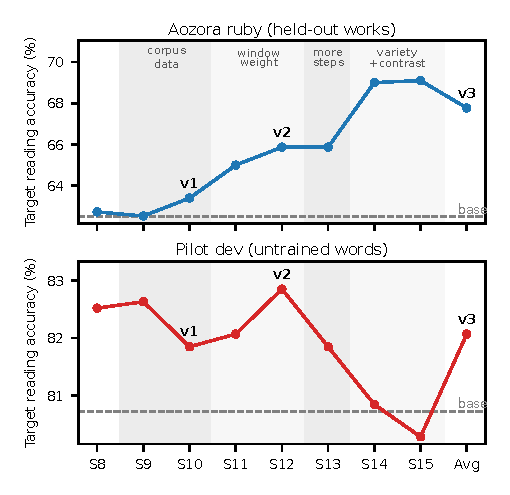
\includegraphics[width=\columnwidth]{fig_progress_en.pdf}
\caption{Held-out accuracy by stage. Aozora improves with window weighting and with sentence
variety. Pilot dev (untrained words) drifts down with long training. Averaging S12 and S15
(``Avg'', released as v3) keeps most of the Aozora gain and restores pilot dev.}
\label{fig:progress}
\end{figure}

\textbf{Loss dilution} (Table~\ref{tab:diag}). After v1, the student fit its hard Wikipedia
and Aozora training rows far worse than the LLM rows (30\%/18\% against 66\%). To find out why,
we trained from the base model on hard rows only, with the same number of passes (24 per row).
Wikipedia rows fit as fast as the LLM rows; the gap came mostly from fewer passes and from long
sentences diluting the target. Weighting the target window helped most. Training 8 layers
instead of 4 also helped, at 1.5$\times$ the cost, and weaker preservation helped least.

\begin{table}[t]
\centering\small
\caption{Fit diagnosis from the base model, with the same number of passes over each set
(accuracy on the training rows, \%).}
\label{tab:diag}
\begin{tabular}{@{}lrrr@{}}
\toprule
Setting & Wikipedia & Aozora & LLM (M3)\\
\midrule
Base & 12.2 & 7.6 & 8.0\\
Recipe of v1 & 34.2 & 18.9 & 35.1\\
+ window weight 5 & \textbf{48.2} & \textbf{28.2} & --\\
+ top 8 layers & 45.0 & 26.6 & --\\
+ preservation $\times0.3$ & 39.2 & 21.7 & --\\
\bottomrule
\end{tabular}
\end{table}

\textbf{Memorization versus variety.}\label{sec:variety} More steps alone (S13) raised the
hard Aozora training rows from 42\% to 57\%. Yet held-out items whose words were trained stayed
at 18\%: the student memorized \emph{sentences}, not word readings. More sentences per word
fixed this. For words that got 6 LLM sentences each (S14), base-misread held-out items were
read correctly 34\% of the time, against 20\% before. Adding 2,000 Aozora works raised newly
covered words from 8\% to 21\%. Words absent from all training data stayed flat at 55\%.

\textbf{Drift and averaging.} Pilot dev (untrained hard words) fell from 82.9\% (S12) to
80.3\% (S15; 11 fixed, 34 broken, $p=8\cdot10^{-4}$). The broken items were mostly untrained
compounds read in odd ways (前庭 マエニワ$\to$ゼンニワ, 活火山 $\to$ イカザン). Common
compounds of the contrast kanji held out from training stayed at 97\% in every model, so this
is a slow drift on untrained words, not a leak of single-kanji readings. Interpolating S12 and
S15 trades the two effects smoothly (Table~\ref{tab:interp}); $\alpha=0.5$ became v3.

\begin{table}[t]
\centering\small
\caption{Interpolating S12 ($\alpha{=}0$) and S15 ($\alpha{=}1$).}
\label{tab:interp}
\begin{tabular}{@{}lrrrr@{}}
\toprule
$\alpha$ & 0 & 0.5 & 0.7 & 1\\
\midrule
Aozora ruby & 65.87 & 67.77 & 68.30 & 69.10\\
Pilot dev & 82.85 & 82.07 & 81.63 & 80.29\\
Wikipedia dev & 85.09 & 84.96 & 84.99 & 85.12\\
\bottomrule
\end{tabular}
\end{table}

\begin{table}[t]
\centering\small
\caption{Released checkpoints, evaluated as exported files. Accuracy (\%) up, CER (\%) down.
v3 vs.\ base (fixed/broken): Aozora 200/49 ($p{=}8\cdot10^{-23}$), Wikipedia 126/66
($p{=}2\cdot10^{-5}$), pilot 31/20 ($p{=}0.16$), JKYB 320/96 ($p{=}3\cdot10^{-29}$).}
\label{tab:release}
\footnotesize\setlength{\tabcolsep}{3.5pt}
\begin{tabular}{@{}lrrrr@{}}
\toprule
& Base & v1 & v2 & v3\\
\midrule
Aozora ruby & 62.50 & 63.30 & 65.80 & \textbf{67.53}\\
Wikipedia dev & 84.04 & 84.37 & \textbf{85.12} & 84.98\\
Pilot dev & 80.73 & -- & \textbf{82.74} & 81.96\\
JSUT kana CER & 1.881 & 1.799 & 1.778 & \textbf{1.713}\\
JVS Whisper CER & \textbf{5.625} & 5.650 & 5.683 & 5.717\\
JKYB-Parakeet & 94.04 & 95.06 & 95.46 & \textbf{95.69}\\
\quad on / kun & 93.0/95.9 & 94.5/96.3 & 95.0/96.5 & 95.2/96.8\\
\bottomrule
\end{tabular}
\end{table}

\textbf{General sentences and robustness.} JSUT kana CER improves in every release
(1.881\%$\to$1.713\%; 161 sentences better, 99 worse). The JVS Whisper CER moves within noise
(13 better, 18 worse), and most of those differences are orthographic variants of the
transcript (時/とき). On JKYB, both halves improve: +1.91\pt{} for the words allowed in early
training and +1.41\pt{} for the held-out half.

\textbf{Seed check.} All other evaluations use seed 0. On the Aozora set with seeds 1 and 2, v3 beats
the base model by +5.73\pt{} with both seeds: 62.27\%$\to$68.00\% (208 fixed, 36 broken) and
62.13\%$\to$67.87\% (209/37). With seed 0 the gain is +5.03\pt.

\section{Discussion}
\textbf{What is learned.} The student learns readings of the words it is trained on, and it
applies them in new sentences once each word has varied contexts. It does not learn
general reading rules: words absent from training do not improve. Coverage therefore comes from
data, and the cheapest data are sentences generated or retrieved for words that the base model
misreads.

\textbf{Limitations.} The evaluation is based on ASR, with one reference voice and one seed
for most sets (see the seed check above), and kana-whisper or the reference readings can be wrong. Listening
was informal. LLM sentences sometimes misuse rare words semantically, even when the reading is
right. The shared BERT couples the text and caption paths, and emoji tokens shift more
(12--14\%) than other tokens. Long continued training drifts on untrained words; averaging
limits this but does not remove it.

\textbf{Other languages.} The recipe needs two things. First, a TTS model whose text encoder
is separate from a frozen acoustic model. Second, an alternative spelling that the frozen model
reads unambiguously. In Japanese, katakana plays this role. Mandarin polyphonic characters
(多音字, e.g.\ 行 \emph{xíng}/\emph{háng}, 长 \emph{cháng}/\emph{zhǎng}) are the analogous
problem for character-input TTS. There, the teacher input could replace the character with an
unambiguous homophone or with pinyin, if the model reads pinyin. Training sentences can come from
polyphone dictionaries and corpora~\cite{g2pm}. We have not tested this.

\section{Conclusion}
Fine-tuning only the top of the text encoder against a kana-reading teacher fixes kanji readings
of a frozen flow-matching TTS without any new speech. The method needs four ingredients:
preservation losses, so that untrained words do not regress; loss weighting on the target
window; varied sentences per word, so that readings generalize beyond memorized sentences; and
checkpoint averaging, to limit drift. With them, the released model improves held-out literary
readings by 5\pt{} and JKYB-Parakeet by 1.7\pt{} without degrading general speech.

\section*{Acknowledgments}
We thank the authors of Irodori-TTS, Echo-TTS, JKYB and its Parakeet edition, kana-whisper,
the JSUT and JVS corpora, Aozora Bunko, Wikipedia, the EDRDG dictionary files, JmdictFurigana,
UniDic, Sudachi and Qwen.

\begin{thebibliography}{99}\footnotesize
\setlength{\itemsep}{0pt}
\bibitem{irodori} C.~Arata. Irodori-TTS: A flow matching-based text-to-speech model with
emoji-driven style control. Hugging Face model \texttt{Aratako/Irodori-TTS-v4.1-Small} and
\url{https://github.com/Aratako/Irodori-TTS}, 2026.
\bibitem{echo} J.~Darefsky. Echo-TTS. Blog post,
\url{https://jordandarefsky.com/blog/2025/echo/}, 2025.
\bibitem{rf} X.~Liu, C.~Gong, Q.~Liu. Flow straight and fast: Learning to generate and transfer
data with rectified flow. \emph{ICLR}, 2023.
\bibitem{fm} Y.~Lipman, R.~T.~Q.~Chen, H.~Ben-Hamu, M.~Nickel, M.~Le. Flow matching for
generative modeling. \emph{ICLR}, 2023.
\bibitem{cfg} J.~Ho, T.~Salimans. Classifier-free diffusion guidance. arXiv:2207.12598, 2022.
\bibitem{dacvae} Meta AI. DACVAE. \url{https://github.com/facebookresearch/dacvae}.
\bibitem{dac} R.~Kumar, P.~Seetharaman, A.~Luebs, I.~Kumar, K.~Kumar. High-fidelity audio
compression with improved RVQGAN. \emph{NeurIPS}, 2023.
\bibitem{modernbert} B.~Warner et al. Smarter, better, faster, longer: A modern bidirectional
encoder for fast, memory efficient, and long context finetuning and inference.
arXiv:2412.13663, 2024.
\bibitem{modernbertja} SB Intuitions. \texttt{sbintuitions/modernbert-ja-310m}. Hugging Face,
2025.
\bibitem{jkyb} SB Intuitions. Joyo Kanji Yomi Benchmark.
\url{https://github.com/sbintuitions/Joyo-Kanji-Yomi-Benchmark}.
\bibitem{jkybp} Parakeet Inc. Joyo Kanji Yomi Benchmark, Parakeet Edition (JKYB-Parakeet).
\url{https://github.com/Parakeet-Inc/Joyo-Kanji-Yomi-Benchmark-Parakeet-Edition}.
\bibitem{kanawhisper} SB Intuitions. \texttt{sbintuitions/kana-whisper}. Hugging Face.
\bibitem{whisper} A.~Radford et al. Robust speech recognition via large-scale weak supervision.
\emph{ICML}, 2023.
\bibitem{jsut} R.~Sonobe, S.~Takamichi, H.~Saruwatari. JSUT corpus: free large-scale Japanese
speech corpus for end-to-end speech synthesis. arXiv:1711.00354, 2017.
\bibitem{jvs} S.~Takamichi et al. JVS corpus: free Japanese multi-speaker voice corpus.
arXiv:1908.06248, 2019.
\bibitem{mcnemar} Q.~McNemar. Note on the sampling error of the difference between correlated
proportions or percentages. \emph{Psychometrika}, 12(2):153--157, 1947.
\bibitem{mecab} T.~Kudo, K.~Yamamoto, Y.~Matsumoto. Applying conditional random fields to
Japanese morphological analysis. \emph{EMNLP}, 2004.
\bibitem{unidic} Y.~Den, J.~Nakamura, T.~Ogiso, H.~Ogura. A proper approach to Japanese
morphological analysis: Dictionary, model, and evaluation. \emph{LREC}, 2008.
\bibitem{sudachi} K.~Takaoka et al. Sudachi: a Japanese tokenizer for business. \emph{LREC}, 2018.
\bibitem{jmdict} J.~Breen. JMdict: a Japanese-multilingual dictionary. \emph{COLING Workshop on
Multilingual Linguistic Resources}, 2004.
\bibitem{jmdictfurigana} Doublevil. JmdictFurigana.
\url{https://github.com/Doublevil/JmdictFurigana}.
\bibitem{qwen3} Qwen Team. Qwen3 technical report. arXiv:2505.09388, 2025.
\bibitem{vllm} W.~Kwon et al. Efficient memory management for large language model serving with
PagedAttention. \emph{SOSP}, 2023.
\bibitem{wiseft} M.~Wortsman et al. Robust fine-tuning of zero-shot models. \emph{CVPR}, 2022.
\bibitem{soups} M.~Wortsman et al. Model soups: averaging weights of multiple fine-tuned models
improves accuracy without increasing inference time. \emph{ICML}, 2022.
\bibitem{g2pm} K.~Park, S.~Lee. g2pM: A neural grapheme-to-phoneme conversion package for
Mandarin Chinese based on a new open benchmark dataset. \emph{Interspeech}, 2020.
\end{thebibliography}
\end{document}
